\documentclass{article}
\usepackage[utf8]{inputenc}
\usepackage[english]{babel}
\usepackage{libertine}
\usepackage[a4paper]{geometry}
\usepackage{parskip}
\usepackage{booktabs}
\usepackage{tabularx}
\usepackage{enumitem}
\usepackage{graphicx}
\usepackage{xcolor}
\usepackage{float}
\usepackage{wrapfig}
\usepackage{multicol}
\usepackage{multirow}
\usepackage{vwcol}
\usepackage{dashrule}
\usepackage{pdfpages}
\usepackage[bottom]{footmisc}

\usepackage{blindtext}

\usepackage{csquotes}
\MakeOuterQuote{"}

\usepackage{hyperref}
\hypersetup{
	pdftitle={Conversion of Singapore Driving Licence -- Munich},
	pdfauthor={Sun Yudong},
	bookmarksnumbered=true,
	bookmarksopen=true,
	bookmarksopenlevel=2,
	pdfstartview=Fit,
	pdfpagemode=UseOutlines,
	colorlinks=true,
	linkcolor=black,
	filecolor=magenta,      
	urlcolor=blue
}
\urlstyle{same}

% Self declared
\newcommand{\blanko}[0]{\textcolor{white}{.}}
\newcommand{\datum}[0]{\today}
% 


\usepackage{fancyhdr}
% Meant to be distributed digitally

\pagestyle{fancy}
\fancyhf{}
\fancyhead[L]{Conversion of Singapore Driving Licence}
\fancyhead[R]{Stand: \datum}
\cfoot{\thepage}

\title{Conversion of Singapore Driving Licence \\ {\large Landeshauptstadt München}}
\author{Sun Yudong}
\date{\datum}

\begin{document}

\maketitle

\section{Introduction}
According to the BMVI\footnote{\url{https://www.bmvi.de/SharedDocs/DE/Artikel/StV/Strassenverkehr/gueltigkeit-auslaendischer-fahrerlaubnisse-in-deutschland.html}} Foreigners from non EU/EEC countries can drive for 6 months with their foreign driving licence after they enter Germany and register their address with the authorities (\de{Anmeldung}). Should you wish to drive beyond that, you will have to convert your licence.\footnote{The author is unfortunately not sure as to whether going back to Singapore and coming back restarts the 6 months.}

To convert your licence, the laws differ from state to state. This document is mainly to document the process the author went through to convert their driving licence here in Munich and serve as an English guide to other Singaporeans coming over to Munich. 

\subsection{Prerequisites}
\begin{enumerate}
    \item You are here on a long term visa (e.g. Work, Study, etc.)
    \item You have done your \de{Anmeldung}
\end{enumerate}

\begin{figure}[H]
    \centering
    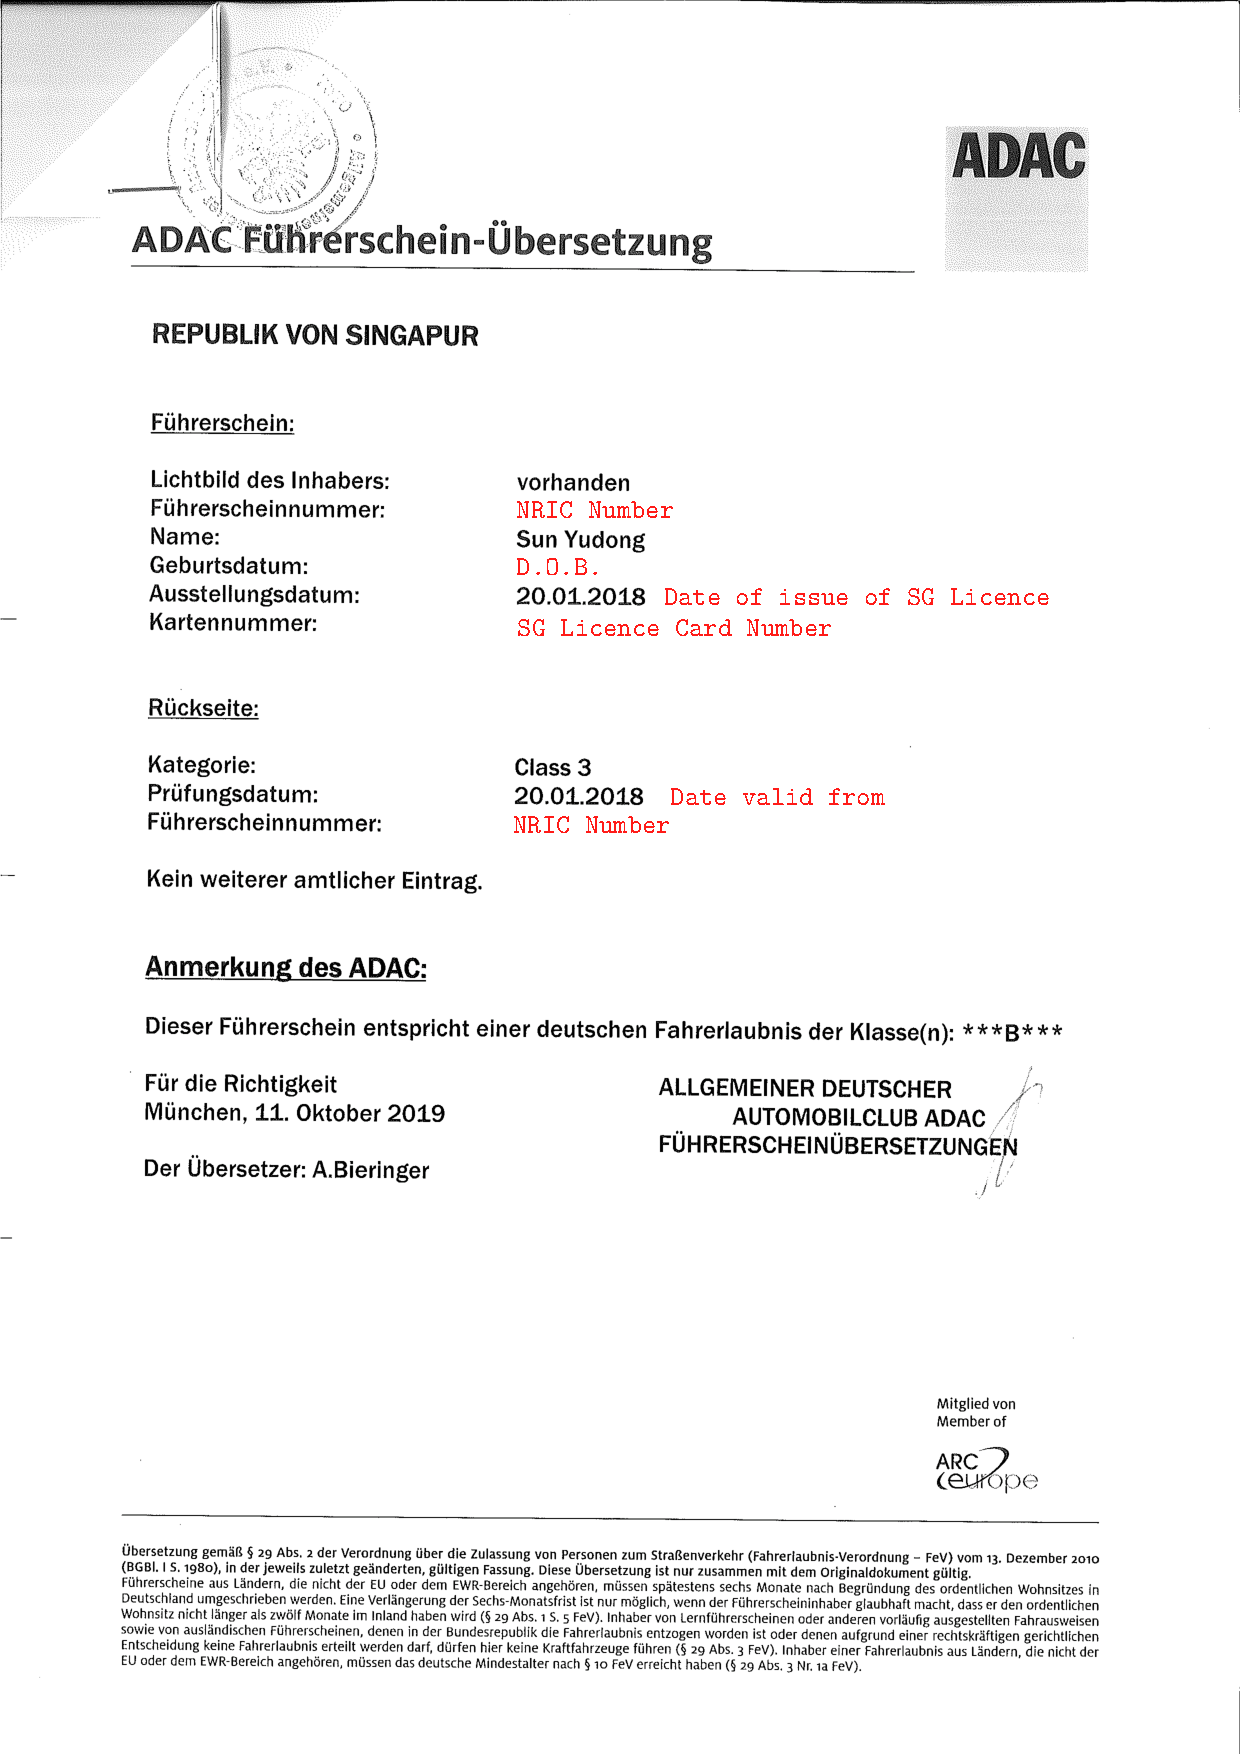
\includegraphics[width=0.7\textwidth]{ADAC.pdf}
    \caption{Translation. This will be submitted to KVR.}
    \label{fig:ADAC Translation}
\end{figure}

You may find more information at the following links. They might be in German:
\begin{itemize}
    \item \url{www.muenchen.de/rathaus/Stadtverwaltung/Kreisverwaltungsreferat/Verkehr/Fuehrerschein.html}
\end{itemize}

\blindtext

\pagebreak 
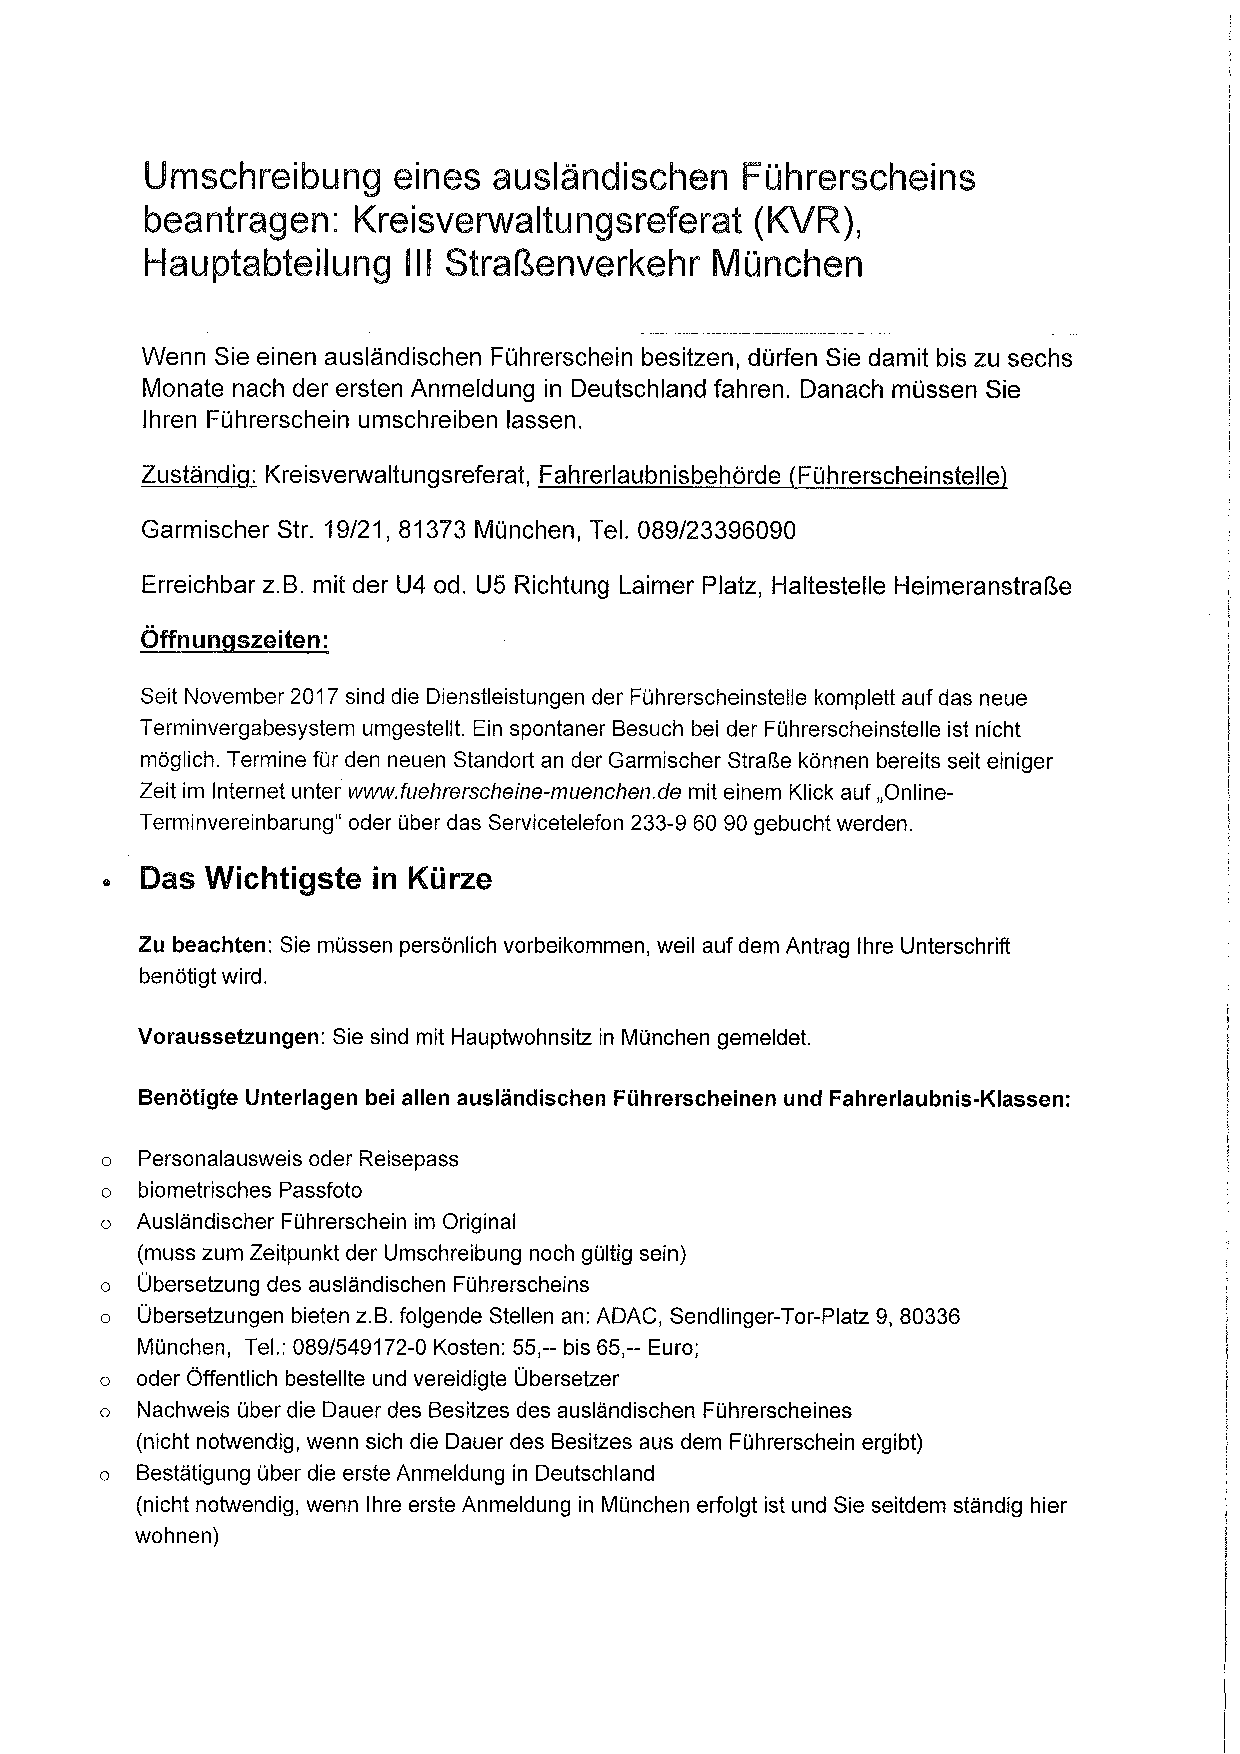
\includepdf[]{ADAC-Infosheet.pdf}
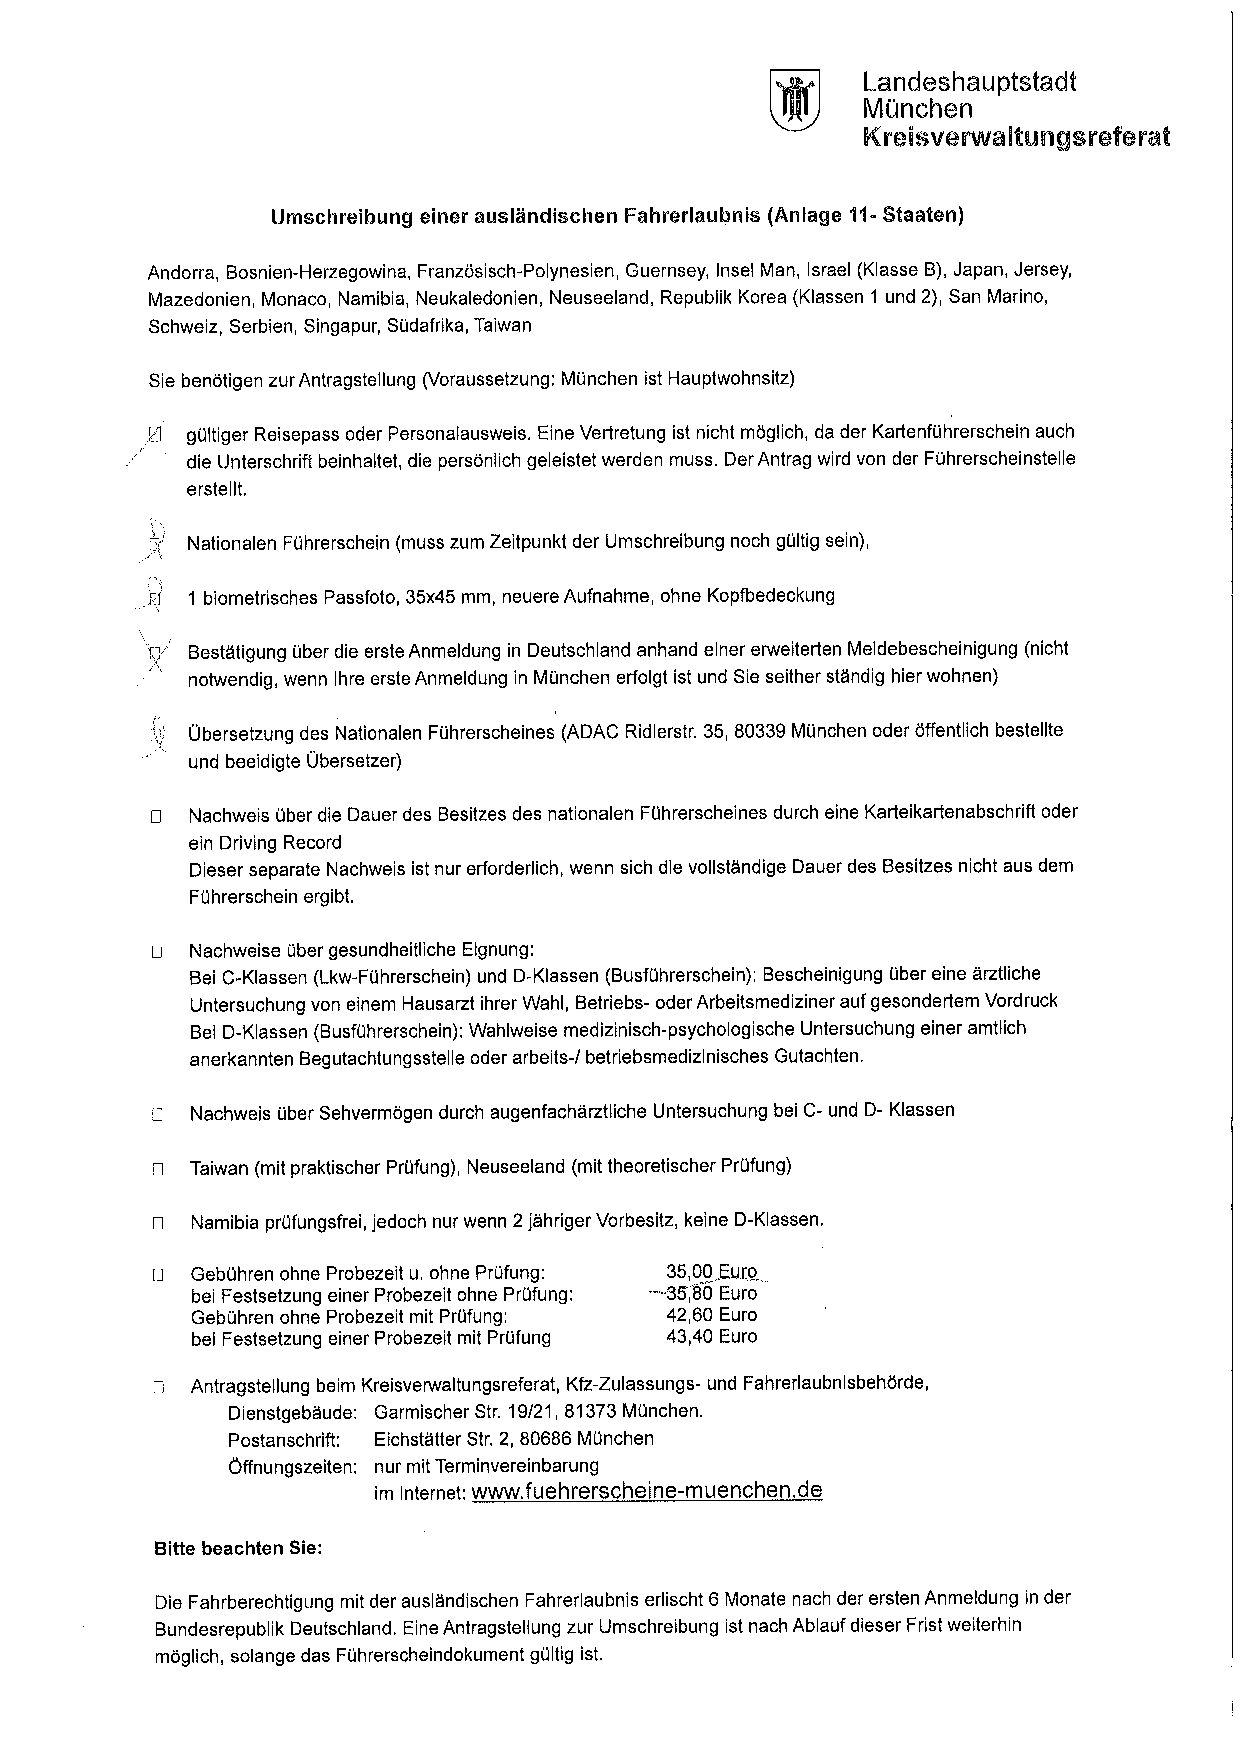
\includepdf[]{KVR-Infosheet.pdf}

\end{document}
